\section{The Gram-Schmidt Orthogonalization Process and Orthogonal Complements} \label{sec 6.2}

In previous chapters, we have seen the special role of the \emph{standard} ordered bases for \(\SET{C}^n\) and \(\SET{R}^n\).
The special properties of these bases stem from the fact that the basis vectors \emph{form an orthonormal set}.
Just as bases are the building blocks of vector spaces, \emph{bases that are also orthonormal sets are the building blocks of inner product spaces}.
We now name such bases.

\begin{definition} \label{def 6.5}
Let \(\V\) be an inner product space.
A subset of \(\V\) is an \textbf{orthonormal basis} for \(\V\) if it is an ordered basis that is orthonormal.
\end{definition}

\begin{note}
為何不跟著定義在上一節最後一個定義就好了...
\end{note}

\begin{example} \label{example 6.2.1}
The standard ordered basis for \(F^n\) is an orthonormal basis for \(F^n\).
(Again in this chapter we assume \(F = \SET{R}\) or \(F = \SET{C}\).)
\end{example}

\begin{example} \label{example 6.2.2}
The set
\[
    \left\{ \left( \frac{1}{\sqrt{5}}, \frac{2}{\sqrt{5}} \right), \left( \frac{2}{\sqrt{5}}, \frac{-1}{\sqrt{5}} \right) \right\}
\]
is an orthonormal basis for \(\SET{R}^2\).
\end{example}

The next theorem and its corollaries illustrate why orthonormal sets and, in particular, orthonormal bases are so important.

\begin{note}
就是用一個標準正交基底來表示任一個向量會變得很簡單的意思。
\end{note}

\begin{theorem} \label{thm 6.3}
Let \(\V\) be an inner product space and \(S = \{ v_1, v_2, ..., v_k \}\) be an orthogonal subset of \(\V\) consisting of nonzero vectors.
If \(y \in \spann(S)\), then
\[
    y = \sum_{i = 1}^k \frac{\LG y, v_i \RG}{\norm{v_i}^2} v_i.
\]
\end{theorem}

\begin{proof}
Write \(y = \sum_{i = 1}^k a_i v_i\), where \(a_1, ..., a_k \in F\).
Then, for \(1 \le j \le k\), we have
\begin{align*}
    \LG y, v_j \RG & = \LG \sum_{i = 1}^k a_i v_i, v_j \RG & \text{by def of \(y\)} \\
        & = \sum_{i = 1}^k a_i \LG v_i, v_j \RG & \text{by \DEF{6.1}(a)(b)} \\
        & \ \RED{=} \ a_j \LG v_j, v_j \RG & \text{since \(S\) is orthogonal} \\
        & = a_j \norm{v_j}^2 & \text{by \DEF{6.3}}
\end{align*}
So \(a_j = \cfrac{\LG y, v_j \RG}{\norm{v_j}^2}\), and the result follows.
\end{proof}

The next corollary follows immediately from \THM{6.3}.

\begin{corollary} \label{corollary 6.3.1}
If, in addition to the hypotheses of \THM{6.3}, \(S\) is ortho\textbf{normal} and \(y \in \spann(S)\), then
\begin{align*}
    y & = \sum_{i = 1}^k \frac{\LG y, v_i \RG}{\norm{v_i}^2} v_i & \text{by \THM{6.3}} \\
      & = \sum_{i = 1}^k \frac{\LG y, v_i \RG}{1} v_i & \text{since \(S\) is orthonormal} \\
      & = \sum_{i = 1}^k \LG y, v_i \RG v_i & \text{of course}
\end{align*}
\end{corollary}

\begin{note}
If \(\V\) possesses a \emph{finite} orthonormal \emph{basis}, then \CORO{6.3.1} allows us to compute the coefficients in a linear combination very easily.
(See \EXAMPLE{6.2.3}.)
\end{note}

\begin{corollary} \label{corollary 6.3.2}
Let \(\V\) be an inner product space, and let \(S\) be an orthogonal subset of \(\V\) consisting of \emph{nonzero} vectors.
Then \(S\) is \emph{\LID{}}.
\end{corollary}

\begin{proof}
Suppose that \(v_1, v_2, ..., v_k \in S\) and
\[
    \sum_{i = 1}^k a_i v_i = \OV.
\]
As in the proof of \THM{6.3} \emph{with \(y = \OV\)}, we have \(a_j = \cfrac{\LG 0, v_j \RG}{\norm{v_j}^2} = \cfrac{0}{\norm{v_j}^2} = 0\) for all \(j\).
So \(S\) is \LID{}.
\end{proof}

\begin{example} \label{example 6.2.3}
By \CORO{6.3.2}, the orthonormal set
\[
     \left\{ \frac{1}{\sqrt{2}}(1, 1, 0), \frac{1}{\sqrt{3}}(1, -1, 1), \frac{1}{\sqrt{6}}(-1, 1, 2) \right\}
\]
obtained in \EXAMPLE{6.1.8} is \LID{} and has three vectors, hence is an orthonormal \emph{basis} for \(\SET{R}^3\).
Let \(x = (2, 1, 3)\).
The coefficients given by \CORO{6.3.1} that express \(x\) as a linear combination of the basis vectors are
\begin{align*}
    a_1 & = \LG (2, 1, 3), \frac{1}{\sqrt{2}}(1, 1, 0) \RG = \frac{3}{\sqrt{2}}\\
    a_2 & = \LG (2, 1, 3), \frac{1}{\sqrt{3}}(1, -1, 1) \RG = \frac{4}{\sqrt{3}} \\
    a_3 & = \LG (2, 1, 3), \frac{1}{\sqrt{6}}(-1, 1, 2) \RG = \frac{5}{\sqrt{6}}
\end{align*}
As a check, we have
\[
    (2, 1, 3) = \frac{3}{\sqrt{2}} \cdot \frac{1}{\sqrt{2}}(1, 1, 0) + \frac{4}{\sqrt{3}} \cdot \frac{1}{\sqrt{3}}(1, -1, 1) + \frac{5}{\sqrt{6}} \cdot \frac{1}{\sqrt{6}}(-1, 1, 2).
\]
\end{example}

\begin{remark} \label{remark 6.2.1}
\CORO{6.3.2} tells us that the vector space \(\textsf{H}\) in \RMK{6.1.8} contains an \emph{infinite} \LID{} set, and hence \(\textsf{H}\) is not a finite-dimensional vector space.
\end{remark}

\begin{remark} \label{remark 6.2.2}
Of course, we have not yet shown that \emph{every} \emph{finite}-dimensional inner product space possesses an \emph{orthonormal} basis.
The next theorem takes us most of the way in obtaining this result.
It tells us how to \emph{construct} an orthogonal set \emph{from a \LID{} set} of vectors in such a way that \textbf{both sets generate the same subspace}.

Before stating this theorem, let us consider a simple case.
Suppose that \(\{ w_1, w2 \}\) is a \LID{} subset of an inner product space (and hence a basis for some \emph{two}-dimensional subspace).
We want to construct an orthogonal set from \(\{ w_1, w_2 \}\) that spans the same subspace.
Figure 6.1 suggests that the set \(\{ v_1, v_2 \}\), where \(v_1 = w_1\) and \(v_2 = w_2 - cw_1\), has this property if \(c\) \emph{is chosen so that} \(v_2\) is orthogonal to \(w_1\).

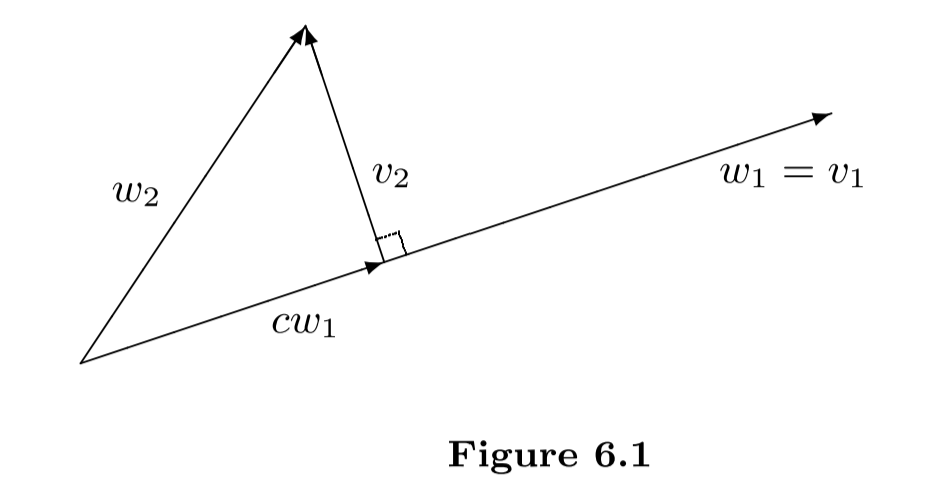
\includegraphics[width=10cm]{images/figure-6-1.png}

To find \(c\), we need only solve the following equation:
\[
    0 = \LG v_2, w_1 \RG = \LG w_2 - cw_1, w_1 \RG = \LG w_2, w_1 \RG - c \LG w_1, w_1 \RG.
\]
So
\[
    c = \frac{\LG w_1, w_2 \RG}{ \norm{w_1}^2 }
\]
Thus
\[
    v_2 = w_2 - c w_1 = w_2 - \frac{\LG w_1, w_2 \RG}{ \norm{w_1}^2 } w_1.
\]
The next theorem shows us that this process can be \emph{extended} to any \emph{finite} linearly independent subset.
\end{remark}

\begin{theorem} [Gram-Schmidt process] \label{thm 6.4}
Let \(\V\) be an inner product space and \(S = \{ w_1, w_2, ..., w_n \}\) be a \LID{} susbet of \(\V\).
Define \(S' = \{ v_1, v_2, ..., v_n \}\), where \(v_1 = w_2\) and
\[
    v_k = w_k - \sum_{j = 1}^{\RED{k - 1}} \frac{\LG \RED{w_k}, v_j \RG}{\norm{v_j}^2} v_j \quad \text{ for } 2 \le k \le n \quad \quad \MAROON{(1)}
\]
Then \(S'\) is an orthogonal set of nonzero vectors such that \(\spann(S') = \spann(S)\).
\end{theorem}

\begin{proof}
The proof is by mathematical induction on \(n\), the \emph{number of vectors in} \(S\).
For \(k = 1, 2, ..., n\), let \(S_k = \{ w_1, w_2, ..., w_k \}\).
If \(n = 1\), then the theorem is proved by taking \(S_1' = S_1\); i.e., \(w_1 = v_1 \ne \OV\).
Assume then that the set \(S'_{k - 1} = \{ v_1, v_2, ..., v_{k-1} \}\) \emph{with the desired properties has been constructed}(i.e. \textbf{induction hypothesis}) by the repeated use of \MAROON{(1)}.
We show that the set \(S'_k = \{ v_1, v_2, ..., v_{k - 1}, v_k \}\) also has the desired properties, where \(v_k\) is obtained from \(S'_{k - 1}\) by \MAROON{(1)}.
If \(v_k = \OV\), then \MAROON{(1)} implies that \(w_k \in \spann(S'_{k - 1})\), which (by induction hypothesis) is equal to \(\spann(S_{k-1})\), which contradicts the assumption that \(S_k\) is \LID{}.
For \(1 \le i \le k- 1\), it follows from \MAROON{(1)} that
\begin{align*}
    \LG v_k, v_i \RG & = \LG w_k - \sum_{j = 1}^{k - 1} \frac{\LG w_k, v_j \RG}{\norm{v_j}^2} v_j, v_i \RG & \text{by \MAROON{(1)}} \\
        & = \LG w_k, v_i \RG - \sum_{j = 1}^{k - 1} \frac{\LG w_k, v_j \RG}{\norm{v_j}^2} \LG v_j, v_i \RG & \text{by \DEF{6.1}(a)(b)} \\
        & = \LG w_k, v_i \RG - \frac{\LG w_k, v_i \RG}{\norm{v_i}^2} \LG v_i, v_i \RG & \text{since \(S'\) is orthogonal by induction hypo} \\
        & = \LG w_k v_i \RG - \frac{\LG w_k, v_i \RG}{\norm{v_i}^2} \norm{v_i}^2 & \text{by \DEF{6.3}} \\
        & = \LG w_k v_i \RG - \LG w_k, v_i \RG = 0 & \text{of course}
\end{align*}
Hence \(S'_k\) is an orthogonal set of nonzero vectors.
Now, by \MAROON{(1)}, we have that \(\spann(S'_k) \subseteq \spann(S_k)\), since each vector in \(S'_k\) can be represented using vectors in \(\spann(S_k)\).
But by \CORO{6.3.2}, (since \(S'_k\) is orthogonal,) \(S'_k\) is \LID{}; so \(\dim(\spann(S'_k)) = k\).
But since \(S_k\) is also \LID{} by supposition (in the description of the theorem), \(\dim(\spann(S_k)) = k\).
Therefore (by \THM{1.11}) \(\spann(S'_k) = \spann(S_k)\).
This closes the induction.
\end{proof}

\begin{remark} \label{remark 6.2.3}
The construction of \(\{ v_1, v_2, ..., v_n \}\) by the use of \THM{6.4} is called the \textbf{Gram-Schmidt process}.
And note that whether a set can be called orthogonal depends on the inner product you choose.
For example, the standard ordered basis for \(F^n\) is an orthogonal(in particular, orthonormal) basis with respect to \emph{standard} inner product.
But it may not be an orthogonal(or orthonormal) basis with respect to other inner product.
\end{remark}

\begin{example} \label{example 6.2.4}
In \(\SET{R}^4\), let \(w_1 = (1, 0, 1, 0), w_2 = (1, 1, 1, 1)\), and \(w_3 = (0, 1, 2, 1)\).
Then \(\{ w_1, w_2, w_3 \}\) is \LID{}.
We use the Gram-Schmidt process to compute the orthogonal vectors \(v_1, v_2\), and \(v_3\), and then we normalize these vectors to obtain an orthonormal set.

Take \(v_1 = w_1 = (1, 0, 1, 0)\).
Then
\begin{align*}
    v_{\RED{2}} & = w_{\RED{2}} - \sum_{j = 1}^{\RED{2} - 1} \frac{\LG w_{\RED{2}}, v_j \RG}{\norm{v_j}^2} v_j & \text{by \THM{6.4}} \\
        & = w_2 - \frac{\LG w_2, v_1 \RG}{\norm{v_1}^2} v_1 \\
        & = (1, 1, 1, 1) - \frac{2}{2}(1, 0, 1, 0) = (0, 1, 0, 1)
\end{align*}
And
\begin{align*}
    v_{\RED{3}} & = w_{\RED{3}} - \sum_{j = 1}^{\RED{3} - 1} \frac{\LG w_{\RED{3}}, v_j \RG}{\norm{v_j}^2} v_j & \text{by \THM{6.4}} \\
        & = w_3 - \frac{\LG w_3, v_1 \RG}{\norm{v_1}^2} v_1 - \frac{\LG w_3, v_2 \RG}{\norm{v_2}^2} v_2 \\
        & = (0, 1, 2, 1) - \frac{2}{2} (1, 0, 1, 0) - \frac{2}{2} (0, 1, 0, 1) = (-1, 0, 1, 0).
\end{align*}
These vectors can be normalized to obtain the ortho\emph{normal} basis \(\{ u_1, u_2, u_3 \}\), where
\begin{align*}
    u_1 & = \frac{1}{\norm{v_1}} v_1 = \frac{1}{\sqrt{2}}(1, 0, 1, 0), \\
    u_2 & = \frac{1}{\norm{v_2}} v_2 = \frac{1}{\sqrt{2}}(0, 1, 0, 1), \\
    u_3 & = \frac{1}{\norm{v_3}} v_3 = \frac{1}{\sqrt{2}}(-1, 0, 1, 0).
\end{align*}
\end{example}

\begin{example} \label{example 6.2.5}
Let \(\V = \POLYRINF\) with the inner product
\[
    \LG f(x), g(x) \RG = \int_{-1}^{1} f(t)g(t) dt,
\]
and consider the subspace \(\POLYRR\) with the \emph{standard} ordered basis \(\beta = \{ w_1, w_2, w_3 \} = \{ 1, x, x^2 \}\).
(Note that, the point is, \(\beta\) may not be an \emph{orthogonal} basis with respect to \emph{this} inner product.)
We use the Gram Schmidt process to replace \(\beta\) by an orthogonal basis \(\{v_1, v_2, v_3 \}\) for \(\POLYRR\), \emph{with respect to} this inner product, and then use this orthogonal basis to obtain an orthonormal basis for \(\POLYRR\).

So by the process, take \(v_1 = 1\).
Then \(\norm{v_1}^2 = \LG 1, 1 \RG = \int_{-1}^1 1 \cdot 1 dt = 2\), and \(\LG x, v_1 \RG = \int_{-1}^1 t \cdot 1 dt = 0\).
Thus
\begin{align*}
    v_2 & = x - \frac{\LG x, v_1 \RG}{\norm{v_1}^2} & \text{by \THM{6.4}} \\
        & = x - \frac{0}{2} = x.
\end{align*}
Furthermore,
\[
    \LG x^2, v_1 \RG = \int_{-1}^1 t^2 \cdot 1 dt = \frac{2}{3} \quad \text{ and } \quad \LG x^2, v_2 \RG = \int_{-1}^1 t^2 \cdot t dt = 0.
\]
Therefore
\begin{align*}
    v_3 & = x^2 - \frac{\LG x^2, v_1 \RG}{\norm{v_1}^2} - \frac{\LG x^2, v_2 \RG}{\norm{v_2}^2} & \text{by \THM{6.4}} \\
        & = x^2 - \frac{1}{3} \cdot 1 - 0 \cdot x \\
        & = x^2 - \frac{1}{3}.
\end{align*}
We conclude that \(\{ 1, x, x^2 - \frac{1}{3} \}\) is an orthogonal basis for \(\POLYRR\) with respect to this inner product.

To obtain an ortho\emph{normal} basis, we normalize \(v_1, v_2\), and \(v_3\) to obtain
\begin{align*}
    u_1 & = \frac{1}{\sqrt{\int_{-1}^1 1^2 dt}} \cdot 1 = \frac{1}{\sqrt{2}}, \\
    u_2 & = \frac{1}{\sqrt{\int_{-1}^1 t^2 dt}} \cdot x = \frac{3}{2} x, \\
    u_3 & = \frac{1}{\sqrt{v_3}} \cdot v_3 = \sqrt{\frac{5}{8}}(3x^2 - 1).
\end{align*}
Thus \(\{ u_1, u_2, u_3 \}\) is the desired orthonormal basis for \(\POLYRR\).
\end{example}

\begin{remark} \label{remark 6.2.4}
Continuing to apply the Gram-Schmidt orthogonalization process to the basis \(\{ 1, x, x^2, ... \}\) for \(\POLYRINF\), we obtain an ortho\emph{gonal} basis \(\{ v_1, v_2, v_3, ... \}\).
For each \(n\), the polynomial
\[
    \frac{1}{v_k(1)} v_k
\]
is called the \(k\)th \textbf{\href{https://www.wikiwand.com/en/Legendre_polynomials\#/Orthogonality_and_completeness}{Legendre polynomial}}.
(Is the scalar \(\frac{1}{v_k(1)}\) used to normalize the orthogonal vector \(v_k\)?)
The first three Legendre polynomials are \(1\), \(x\) and \(\frac{1}{2} (3x^2 - 1)\).
The set of Legendre polynomials is also an orthogonal basis for \(\POLYRINF\).
\end{remark}

The following result gives us a simple method of representing a vector as a linear combination of the vectors in an ortho\emph{normal} basis.

\begin{theorem} \label{thm 6.5}
Let \(\V\) be a nonzero \emph{finite}-dimensional inner product space.
Then \(\V\) \textbf{has} an orthonormal basis \(\beta\).
Furthermore. if \(\beta = \{ v_1, v_2, ..., v_n \}\) and \(x \in \V\), then
\[
    x = \sum_{i = 1}^n \LG x, v_i \RG v_i.
\]
\end{theorem}

\begin{note}
無限維度有標準正交基底也需要選擇公里或\ Zorn's Lemma.
\end{note}

\begin{proof}
Let \(\beta_0\) be an ordered basis for \(\V\).
Apply \THM{6.4} to obtain an orthogonal \emph{set} \(\beta'\) of nonzero vectors with \(\spann(\beta') = \spann(\beta_0) = \V\).
By normalizing each vector in \(\beta'\), we obtain an orthonormal \emph{set} \(\beta\) that generates \(\V\).
By \CORO{6.3.2}, \(\beta\) is \LID{}; therefore \(\beta\) is an orthonormal \emph{basis} for \(\V\).
The remainder of the theorem follows from \CORO{6.3.1}.
\end{proof}

\begin{example} \label{example 6.2.6}
We use \THM{6.5} to represent the polynomial \(f(x) = 1 + 2x + 3x^2\) as a linear combination of the vectors in the orthonormal basis \(\{ u_1, u_2, u_3 \}\) for \(\POLYRR\) obtained in \EXAMPLE{6.2.5}.
Observe that
\[
    \LG f(x), u_1 \RG = \int_{-1}^{1} \frac{1}{\sqrt{2}} (1+2 t+3 t^2) \cdot 1 dt = 2 \sqrt{2} \\
    \LG f(x), u_2 \RG = \int_{-1}^{1} \sqrt{\frac{3}{2}} (1+2 t+3 t^2) \cdot t dt = \frac{2 \sqrt{6}}{3}
\]
and
\[
    \LG f(x), u_3 \RG = \int_{-1}^{1} \sqrt{\frac{5}{8}} (1 + 2t + 3t^2) (3 t^2 - 1) d t = \frac{2 \sqrt{10}}{5}.
\]
Therefore \(f(x) = 2 \sqrt{2} u_1 + \frac{2 \sqrt{6}}{3} u_2 + \frac{2 \sqrt{10}}{5} u_3\).
\end{example}

\THM{6.5} gives us a simple method for computing the entries of the \textbf{matrix representation} of a linear operator \textbf{with respect to an orthonormal basis}.

\begin{corollary} \label{corollary 6.5.1}
Let \(\V\) be a \emph{finite}-dimensional inner product space with an \emph{orthonormal} basis \(\beta = \{ v_1, v_2, ..., v_n \}\).
Let \(\T\) be a linear operator on \(\V\), and let \(A = [\T]_{\beta}\).
Then for any \(i\) and \(j\), \(A_{ij} = \LG \T(v_j), v_i \RG\).
(Notice the order of \(i\) and \(j\) in the equation.)
\end{corollary}

\begin{proof}
In particular from \THM{6.5}, we have
\[
    \T(v_j) = \sum_{i = 1}^n \LG \T(v_j), v_i \RG v_i.
\]
Hence \(A_{ij} = \LG \T(v_j), v_i \RG\).
\end{proof}

\begin{remark} \label{remark 6.2.5}
The scalars \(\LG x, v_i \RG\) given in \THM{6.5} have been studied \emph{extensively} for special inner product spaces. 
Although the vectors \(v_1, v_2, ..., v_n\) were chosen from an orthonormal basis, we introduce a terminology associated
with orthonormal sets \(\beta\) in more general inner product spaces.
\end{remark}

\begin{definition} \label{def 6.6}
Let \(\beta\) be an orthonormal subset (possibly infinite) of an inner product space \(\V\), and let \(x \in \V\).
We define the \textbf{Fourier coefficient\RED{s}} of \(x\) relative to \(\beta\) to be the scalars \(\LG x, y \RG\), where \(y \in \beta\).
\end{definition}

\begin{remark} \label{remark 6.2.6}
In the first half of the 19th century, the French mathematician Jean Baptiste Fourier was associated with the study of the \emph{scalars} (for any integer \(n\))
\[
    \int_0^{2\pi} f(t) \sin nt dt \quad \text{ and } \quad \int_0^{2\pi} f(t) \cos nt dt
\]
or in the complex case,
\[
    c_n = \frac{1}{2\pi} f(t) e^{-\iu n t} dt.
\]
for a function \(f\).
In the context of \EXAMPLE{6.1.9}, we see that \(c_n = \LG f, f_n \RG\), where \(f_n(t) = e^{\iu nt}\); that is, \(c_n\) is the nth \emph{Fourier coefficient} for a continuous function \(f \in \textsf{H}\) relative to \(S\).
The coefficients \(c_n\) are the ``classical'' Fourier coefficients of a function, and the literature concerning their behavior is extensive.
We learn more about Fourier coefficients in the remainder of this chapter.
\end{remark}

\begin{example} \label{example 6.2.7}
Let \(S = \{ e^{\iu n t} : n \text{ is an integer} \}\).
In \EXAMPLE{6.1.9}, \(S\) was shown to be an orthonormal set in \(\textsf{H}\).
We compute the Fourier coefficients of \(f(t) = t\) relative to \(S\).
Using \emph{integration by parts}, we have, for \(n \ne 0\),
\[
    \LG f, f_n \RG = \frac{1}{2\pi} \int t \conjugatet{e^{\iu n t}} dt = \int \frac{1}{2\pi} t e^{-\iu n t} dt = \frac{-1}{\iu n}, \quad \MAROON{(1)}
\]
and, for \(n = 0\),
\[
    \LG f, f_n \RG = \LG f, e^0 \RG = \LG f, 1 \RG = \int \frac{1}{2\pi} t \cdot 1 dt = \pi. \quad \MAROON{(2)}
\]
As a result of these computations, and using \EXEC{6.2.16}, we obtain an \emph{upper bound} for the sum of a special \emph{infinite series} as follows:
\begin{align*}
    \norm{f}^2 & \ge \sum_{n = -k}^k \abs{ \LG f, f_n \RG }^2 \\
        & = \sum_{n = -k}^{-1} \abs{ \LG f, f_n \RG }^2 + \abs{ \LG f, 1 \RG }^2 + \sum_{n = 1}^k \abs{f, f_n}^2 \\
        & = \sum_{n = -k}^{-1} \frac{1}{n^2} + \pi^2 + \sum_{n = 1}^k \frac{1}{n^2} & \text{by using \MAROON{(1)(2)}} \\
        & = 2 \sum_{n = 1}^k \frac{1}{n^2} + \pi^2 & \text{of course}
\end{align*}
for every \(k\).

Now, using the fact that \(\norm{f}^2 = \frac{4}{3}\pi^2\), we obtain
\[
    \frac{4}{3}\pi^2 \ge 2 \sum_{n = 1}^k \frac{1}{n^2} + \pi^2,
\]
or
\[
    \frac{\pi^2}{6} \ge \sum_{n = 1}^k \frac{1}{n^2}.
\]
Because this inequality holds for all \(k\), we may let \(k \to \infty\) to obtain
\[
    \frac{\pi^2}{6} \ge \sum_{n = 1}^{\infty} \frac{1}{n^2}.
\]
Additional results may be produced by replacing \(f\) by other functions.
\end{example}

We are now ready to proceed with the concept of an \emph{orthogonal complement}.

\begin{definition} \label{def 6.7}
Let \(S\) be a nonempty subset of an inner product space \(\V\).
We define \(S^{\perp}\) (read ``\(S\) perp'') to be the set of all vectors \textbf{in \(\V\)} that are \emph{orthogonal} to every vector in \(S\);
that is, \(S^{\perp} = \{ x \in \V: \LG x, y \RG = 0 \text{ for all } y \in S\}\).
The set \(S^{\perp}\) is called the \textbf{orthogonal complement} of \(S\).

It is easily seen that \(S^{\perp}\) is a subspace of \(\V\) for any subset \(S\) of \(\V\).
And of course from the definition, \(S \cap S^{\perp} = \{ \OV \}\).
\end{definition}

\begin{example} \label{example 6.2.8}
The reader should verify that \(\{ \OV \}^{\perp} = \V\) and \(\V^{\perp} = \{ \OV \}\) for any inner product space \(\V\).
\end{example}

\begin{example} \label{example 6.2.9}
If \(\V = \SET{R}^3\) and \(S = \{ e_3 \}\), then \(S^{\perp}\) equals the \(xy\)-plane (see \EXEC{6.2.5}).
\end{example}

\EXEC{5.1.18} provides an interesting example of an orthogonal complement in an \emph{infinite}-dimensional inner product space. 
\begin{remark} \label{remark 6.2.7}
Consider the problem in \(\SET{R}^3\) of finding the distance from a point \(P\) to a plane \(\W\).
(Well this is high school algebra.)
(See Figure 6.2.)

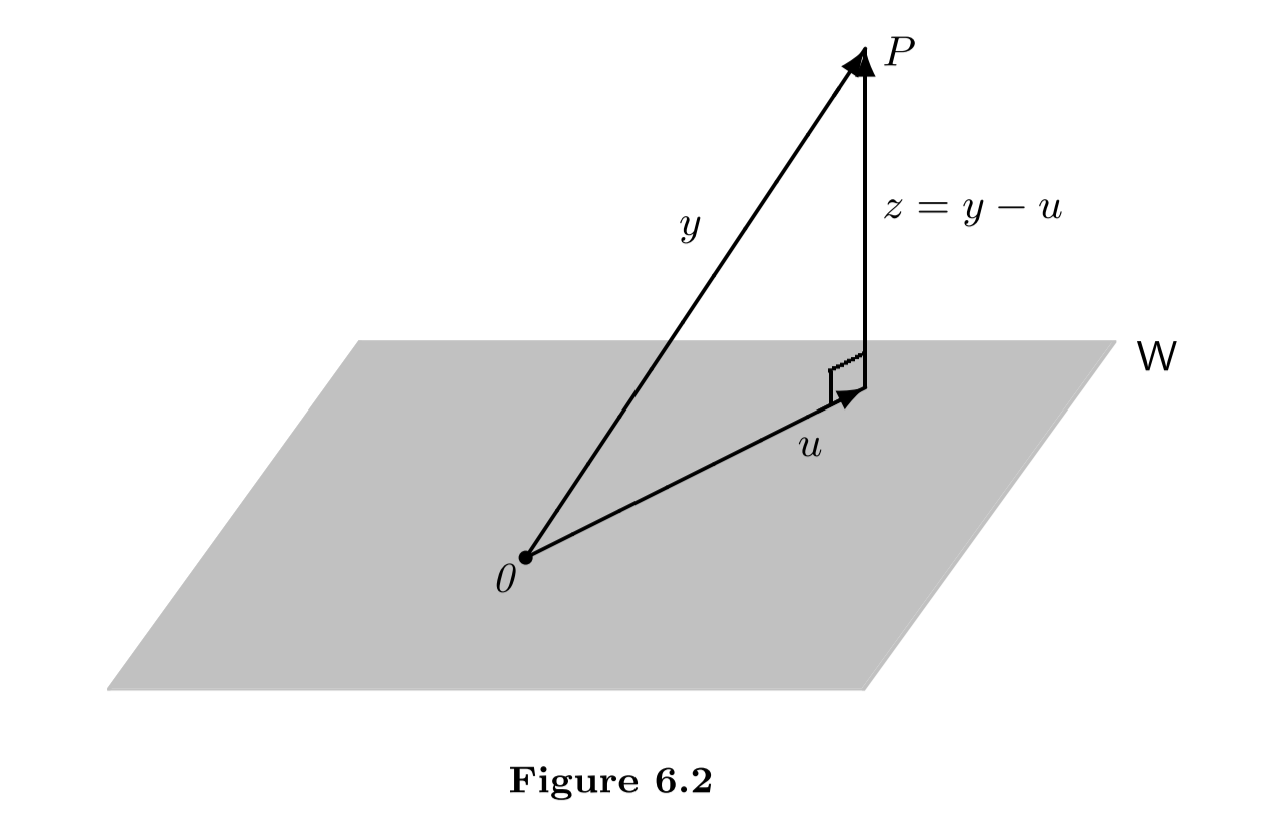
\includegraphics[width=12cm]{images/figure-6-2.png}

Problems of this type arise in many settings.
If we let \(y\) be the vector determined by \(0\) and \(P\).
We may restate the problem as follows:
Determine the vector \(u\) in \(\W\) that is ``\textbf{closest}'' to \(y\).
The desired distance is clearly given by \(\norm{y - u}\).
\emph{Notice} from the figure that the vector \(z = y - u\) is \emph{orthogonal} to \textbf{every vector} in \(\W\), and so \(z \in \W^{\perp}\).

The next result presents a practical method of finding \(u\) in the case that \(\W\) is a \emph{finite}-dimensional \emph{subspace} of an inner product space.
\end{remark}

\begin{theorem} \label{thm 6.6}
Let \(\W\) be a finite-dimensional subspace of an inner product space \(\V\), and let \(y \in \V\).
Then \emph{there exist} \textbf{unique} vector \(u \in \W\) and \textbf{unique} vector \(z \in \W^{\perp}\), such that \(y = u + z\).
Furthermore, if \(\{ v_1, v_2, ..., v_k \}\) is an orthonormal basis \textbf{for \(\W\)}, then
\[
    u = \sum_{i = 1}^k \LG y, v_i \RG v_i.
\]
\end{theorem}

\begin{note}
\THM{6.6} 就是最廣義的看法:
給定一個子空間,然後給定一個向量\ \(y\),這個向量\ \(y\) 可以拆成一組\textbf{唯一的}表示法\ \(u + z\),使得\ \(u\) 在該子空間,\(z\) 在子空間的正交補集內。
如果是 \(\SET{R}^3\) 的例子就會是\ Figure 6.2。
\end{note}

\begin{proof}
Let \(\{ v_1, v_2, ..., v_k \}\) be an orthonormal basis for \(\W\), let \(u\) be as defined in the preceding equation, and let \(z = y - u\). Clearly \(u \in \W\) and \(y = u + z\).

To show that \(z \in \W^{\perp}\), it suffices to show, by \EXEC{6.2.7}, that \(z\) is orthogonal to each \(v_j\).
For any \(j\), we have
\begin{align*}
    \LG z, v_j \RG & = \LG y - u, v_j \RG = \LG y - \sum_{i = 1}^k \LG y, v_i \RG v_i, v_j \RG & \text{of course} \\
        & = \LG y, v_j \RG - \sum_{i = 1}^k \LG y, v_i \RG \LG v_i, v_j \RG & \text{by \DEF{6.1}(a)(b)} \\
        & = \LG y, v_j \RG - \LG y, v_{\RED{j}} \RG \LG v_{\RED{j}}, v_j \RG & \text{since \(v_i\)'s are in particular orthogonal} \\
        & = \LG y, v_j \RG - \LG y, v_{j} \RG \norm{v_j}^2 & \text{by \DEF{6.3}} \\
        & = \LG y, v_j \RG - \LG y, v_{j} \RG \cdot 1 = \LG y, v_j \RG - \LG y, v_{j} \RG & \text{since \(v_i\)'s are ortho\emph{normal}} \\
        & = 0.
\end{align*}
Hence \(z \in \W^{\perp}\), hence the existence part that \(y = u + z\) where \(u \in \W\) and \(z \in \W^{\perp}\) is showed.

Now for the uniqueness part, suppose that \(y = u + z = u' + z'\), where \(u' \in \W\) and \(z' \in \W^{\perp}\).
Then \(u - u' = z'- z\), where \(u - u' \in \W\) and \(z' - z \in \W^{\perp}\), and the equation implies they both \(\in \W \cap \W^{\perp}\).
But by \DEF{6.7}, \(\W \cap \W^{\perp} = \{ \OV \}\), hence \(u - u' = z' - z = \OV\), hence \(u = u'\) and \(z = z'\), showing the uniqueness.
\end{proof}

\begin{corollary} \label{corollary 6.6.1}
In the notation of \THM{6.6}, the vector \(u\) is the unique vector in \(\W\) that is ``closest'' to \(y\);
that is, for any \(x \in \W\), \(\norm{y - x} \ge \norm{y - u}\), and this inequality is an equality if and only if \(x = u\).
\end{corollary}

\begin{proof}
As in \THM{6.6}, we have that \(y = u + z\), where \(z \in \W^{\perp}\).
Let \(x \in \W\).
Then \(u - x\) is orthogonal to \(z\), so, by \EXEC{6.1.10}, we have
\begin{align*}
    \norm{y - x}^2 & = \norm{(u + z) - x}^2 = \norm{(u - x) + z^2} & \text{tricky but of course} \\
        & = \norm{u - x}^2 + \norm{z}^2 & \text{by \EXEC{6.1.10}} \\
        & \ge \norm{z}^2 & \text{by \THM{6.2}(b), \(\norm{u - x}^2 \ge 0\)} \\
        & = \norm{y - u}^2, & \text{of course}
\end{align*}
which implies \(\norm{y - x} \ge \norm{y - u}\).

Now suppose that \(\norm{y - x} = \norm{y - u}\).
Then the inequality above becomes an equality, and therefore \(\norm{u - x}^2 + \norm{z}^2 = \norm{z}^2\).
It follows that \(\norm{u - x} = 0\), and hence (by \THM{6.2}(a)) \(x = u\).

For the converse, if \(x = u\), then of course \(y - x = y - u\) hence of course \(\norm{y - x} = \norm{y - u}\).
\end{proof}

\begin{additional definition} \label{adef 1.3}
The vector \(u\) in the corollary is called the \textbf{orthogonal projection} of \(y\) on \(\W\).
We will see the importance of orthogonal projections of vectors in the application to \emph{least squares} in \SEC{6.3}.
\end{additional definition}

\begin{example} \label{example 6.2.10}
Let \(\V = \POLYRRR\) with the inner product
\[
    \LG f(x),g(x) \RG = \int_{-1}^{1} f(t)g(t) dt
\]
for all \(f(x), g(x) \in \V\).
We compute the orthogonal projection of \(f(x) = x^3\) on \(\POLYRR\).
Let it be \(f_1(x)\).

By \EXAMPLE{6.2.5},
\[
    \{ u_1, u_2, u_3 \} = \left\{ \frac{1}{\sqrt{2}}, \frac{3}{2} x, \sqrt{\frac{5}{8}}(3x^2 - 1) \right\}
\]
is an orthonormal basis for \(\POLYRR\).
By \THM{6.6}, we need to compute \(\LG f(x), u_1 \RG, \LG f(x), u_2 \RG\) and \(\LG f(x), u_3 \RG\).
So we have
\[
    \LG f(x), u_1 \RG = \int_{-1}^{1} t^3 \frac{1}{\sqrt{2}} dt = 0,
    \quad \LG f(x), u_2 \RG = \int_{-1}^{1} t^3 \sqrt{\frac{3}{2}} t dt = \frac{\sqrt{6}}{5}
\]
and
\[
    \LG f(x), u_3 \RG = \int_{-1}^{1} t^{3} \sqrt{\frac{5}{8}} (3 t^2 - 1) dt = 0
\]
Hence
\begin{align*}
    f_{1}(x) & = \LG f(x), u_1 \RG u_1 + \LG f(x), u_2 \RG u_2 + \LG f(x), u_3 \RG u_3 & \text{by \THM{6.6}} \\
        & = \frac{\sqrt{6}}{5} \cdot \sqrt{\frac{3}{2}}x = \frac{3}{5} x & \text{replacing variables}
\end{align*}
\end{example}

\begin{remark} \label{remark 6.2.8}
It was shown in \CORO{1.10.2}(corollary to the replacement theorem) that any \LID{} set in a \emph{finite}-dimensional vector space can be extended to a basis.
The next theorem provides an interesting analog for an orthonormal subset of a \emph{finite}-dimensional inner product space.
\end{remark}

\begin{theorem} \label{thm 6.7}
Suppose that \(S = \{ v_1, v_2, ..., v_k \}\) is an orthonormal set in an \(n\)-dimensional inner product space \(\V\).
Then
\begin{enumerate}
\item \(S\) can be extended to an \textbf{orthonormal} basis \(\{ v_1, v_2, ..., v_k, v_{k+1}, ..., v_n \}\) for \(\V\).
\item If \(\W = \spann(S)\), then \(S_1 = \{v_{k+1}, v_{k+2}, ..., v_n \}\) is an orthonormal basis for \(\W^{\perp}\).
    (using the preceding notation).
\item If \(\W\) is any \emph{subspace} of \(\V\), then \(\dim(\V) = \dim(\W) + \dim(\W^{\perp})\).
\end{enumerate}
\end{theorem}

\begin{proof} \ 

\begin{enumerate}
\item By \CORO{1.10.2}, \(S\) can be extended to an \emph{ordered basis} \(S' = \{ v_1, v2, ..., v_{k}, w_{k+1}, ..., w_n \}\) for \(\V\).
Now apply the Gram-Schmidt process to \(S'\).
The first \(k\) vectors resulting from this process \textbf{are the vectors in \(S\)} by \EXEC{6.2.8}, and this new set spans \(\V\).
Normalizing the last \(n - k\) vectors of this set produces an orthonormal set that spans \(\V\).
The result now follows.

\item Because \(S_1\) is a subset of a (orthonormal) basis, it is \LID{}.
And for every vector in \(S_1\), it is orthogonal to every vector in \(S\), hence is orthogonal to every vector in \(\spann(S) = \W\), so by \DEF{6.7} it is in \(\W_{\perp}\), hence \(S_1 \subseteq \W_{\perp}\).
So we need only show that it spans \(\W_{\perp}\).
Note that, for any \(x \in \V\), since \(\{ v_1, v_2, ..., v_n\) is an orthonormal basis, (by \THM{6.5}) we have
\[
    x = \sum_{i = 1}^n \LG x, v_i \RG v_i.
\]
Now if \(x\) is also in \(\W^{\perp}\), then \(\LG x, v_i \RG = 0\) for \(1 \le i \le k\).
Therefore
\[
    x = \sum_{i = k + 1}^n \LG x, v_i \RG v_i \in \spann(S_1).
\]

\item Let \(\W\) be a subspace of \(\V\).
It is a \emph{finite}-dimensional inner product space because \(\V\) is, and so it has an orthonormal basis \(\{ u_1, u_2, ..., u_k \}\).
By (a) and (b). we have
\begin{align*}
    & \dim(\V) \\
    & = n = k + (n - k) & \text{of course} \\
    & = \dim(\W) + (n - k) & \text{\(\{ u_1, ..., u_k \}\) is a basis for \(\W\)} \\
    & = \dim(\W) + \dim(\W^{\perp}) & \text{by (a)(b), the extended \(\{ u_{k + 1}, ..., u_{n} \}\) is a basis for \(\W^{\perp}\)}
\end{align*}
\end{enumerate}
\end{proof}

\begin{example} \label{example 6.2.11}
Let \(\W = \spann(\{ e_1, e_2 \})\) in \(F^3\).
Then \(x = (a, b, c) \in \W^{\perp}\) if and only if \(0 = \LG x, e_1 \RG = a\) and \(0 = \LG x , e_2 \RG = b\).
So \(x = (0, 0, c)\), and therefore \(\W^{\perp} = \spann(\{ e_3 \})\).
One can deduce the same result by noting that \(e_3 \in \W^{\perp}\) and, from \THM{6.7}(c), that \(\dim(\W^{\perp}) = \dim(V) - \dim(W) = 3 - 2 = 1\).
\end{example}
